\chapter{Local Interpretable Model-agnostic Explanations (LIME)}

Local Interpretable Model-agnostic Explanations (LIME) \citep{ribeiro2016whyitrustyou}  is a tool used to visualize the importance of features on the result of a model's prediction.
A score is given to each feature fed to the model, making it possible to understand a black-box model's decision based on its inputs. 

In this chapter, we will discuss how LIME works, how can one use it on image classification models, we will present our implementation of the method and show some experiments done using the technique. 

\section{How it Works}

LIME works by training an interpretable model (\ref{sec:what_is_xai}) to mock the complex \emph{black-box} model over a region of the model's domain.
The underlying idea is that while the model's decision boundary across the entire domain may be complex, it tends to be simpler within smaller, localized regions.

\begin{figure} 
    \centering
    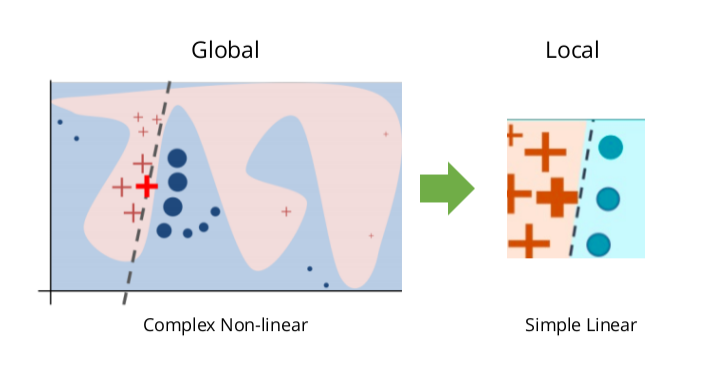
\includegraphics[width=0.5\linewidth]{figuras/lime_regions.png}
    \caption{Smaller regions of model's decion boundary tend to have simple, linear behaviour. Font: C3.ai\footnotemark}
\end{figure}
\footnotetext{https://c3.ai/glossary/data-science/lime-local-interpretable-model-agnostic-explanations/}

To train the interpretable model, a single sample is selected and small perturbations are applied to that data point in order to create a dataset, consisting of the sample image and its perturbations.
Using the dataset, the interpretable model is trained by minimizing the optimization problem bellow:

\begin{equation}
    g^* = \argmin_{g \;\in\; G} \mathcal{L}(f, g, \pi_x) + \Omega(g).
    \label{eq:lime_optimization}  
\end{equation}

Where \(g^*\) is the final trained interpretable model, 
\(G\) is a set of interpretable models, \(f\) is the black-box model, 
\(\Omega\) is a function that maps a model's complexity to a number, with higher complexity yielding higher numbers (Used to penalize complexity in models used to mock the black-box model),
\(\pi_x\) is a function to penalize samples in the dataset "too far" from the original sample \(x\) and
\(\mathcal{L}\) is a cost function to quantify the similarity between the interpretable model's decisions and the complex model's decisions, defined by the expression bellow:

\begin{equation}
    \mathcal{L}(f, g, \pi_x) = \sum_{z, z' \in \; Z} \pi_x(z) (f(z) - g(z'))^2.
    \label{eq:lime_loss}  
\end{equation}

Where \(Z\) is the artificial dataset created from the sample, with datapoints \(z\) - a point with the original model's features, and \(z'\), a data point that represents a transformation applied to those features, like using a subset of inputs or attributes created by \emph{feature engineering}.

Because of the huge ammount of variables in a image classification task, directly using an image consisting of hundreds of thousands of pixels in an interpretable model would yield poor results, since analyzing each individual pixel's contribution to a prediction is not well aligned with a human interpretation of image features.
In order to generate more valuable results, a feature engineering technique will be proposed on the next section to model LIME for Image classification tasks. 

\section{LIME on Image Models}

\section{Implementation}


\section{Experiments} 